% Copyright (c) 2014,2016 Casper Ti. Vector
% Public domain.

\chapter{背景}
%\pkuthssffaq % 中文测试文字。
\section{Rust 编程语言}
Rust\parencite{matsakis2014rust} 是一种由 Mozilla 开发的系统级编程语言,于 2010 年首次发布。
它被设计为一种安全、并发和实用的编程语言,旨在解决 C / C++ 中存在的一些常见问题,如内存安全性和并发性。
Rust 的设计理念包括“零成本抽象”和“保证内存安全”,使得开发者能够编写高性能且安全的软件。

在“保障内存安全”方面,Rust 引入了所有权系统\parencite{rust_owner}\parencite{rust_owner1} 、
引用\parencite{rust_ref} 和生命周期\parencite{rust_lifetime}\parencite{rust_lifetime1} 等特性,
在编译期就检查出潜在的安全问题。
通过所有权系统,Rust 在编译时进行内存管理,避免了常见的内存错误,如空指针引用和数据竞争。
在 Rust 中,每个值都有一个所有者,该所有者负责释放其值的内存。
当所有者超出作用域时,其值的内存将被自动释放,从而避免了内存泄漏。
此外,Rust 还引入了引用(references)的概念,允许在不转移所有权的情况下访问值。
创建一个引用的行为称为借用,借用规则确保在编译时避免数据竞争和内存错误,使得 Rust 程序更加安全和可靠。
生命周期检查则确保引用的有效性,防止出现悬垂引用和数据竞争等问题,提高了代码的安全性和可靠性。

而在“零成本抽象”方面,Rust 引入了模式匹配\parencite{rust_match}、枚举类型\parencite{rust_enum}和 trait\parencite{rust_trait} 等功能,使得代码编写更加简洁和易读,在操作系统设计中更是如此。
模式匹配是 Rust 中强大的特性之一,可以根据数据的结构和内容进行匹配和解构。
在操作系统设计中,模式匹配可以用于处理各种不同的系统状态、事件和数据结构。
通过模式匹配,开发者可以根据不同的情况编写相应的处理逻辑,使得操作系统代码更加清晰、健壮和易于维护。
枚举类型在操作系统设计中可以用于表示系统中的不同状态、类型和变体。
通过枚举类型,可以定义系统中的各种数据结构和状态转换,使得代码更加结构化和可靠。
在操作系统内核中,枚举类型可以用来表示不同的系统调用、错误类型、进程状态等,帮助开发者更好地组织和管理系统的复杂性。
而 trait 是 Rust 中的一种抽象机制,类似于其他语言中的接口或抽象类,可以定义共享的行为和功能。
在操作系统设计中,trait 可以用于定义各种系统组件的通用行为,使得代码更具灵活性和可复用性。

由于其出色的性能、安全性和并发性,Rust 在诸多领域得到广泛应用,包括系统编程\parencite{balasubramanian2017system} 、
嵌入式开发\parencite{borgsmuller2021rust} 、网络服务\parencite{chanda2018network} 和区块链\parencite{rusch2019themis} 等。
随着时间的推移,Rust 社区不断壮大,许多开发者和组织纷纷采用 Rust 来构建高效且可靠的软件系统。
Asterinas 也正是看中了 Rust 的这些优势,选择 Rust 作为主要的开发语言。

\section{exFAT 文件系统}
\subsection{exFAT 文件系统概述}
exFAT (Extended File Allocation Table)\parencite{exFAT}\parencite{exFAT1}\parencite{exFAT2}是由微软公司开发的一种文件系统,
专为闪存存储,如 USB 闪存驱动器、SD 卡和 CF 卡等设计。作为 FAT32\parencite{russinovich2009windows} 的后继文件系统,
exFAT 主要解决了 FAT32 在处理大文件和大容量存储设备上的限制。具体来说,
exFAT 文件系统使用64位来描述文件大小,从而支持依赖于非常大的文件的应用程序;
exFAT 文件系统还允许最大32MB的簇,有效地支持了非常大的存储设备。

\begin{figure}[h]
    \centering
    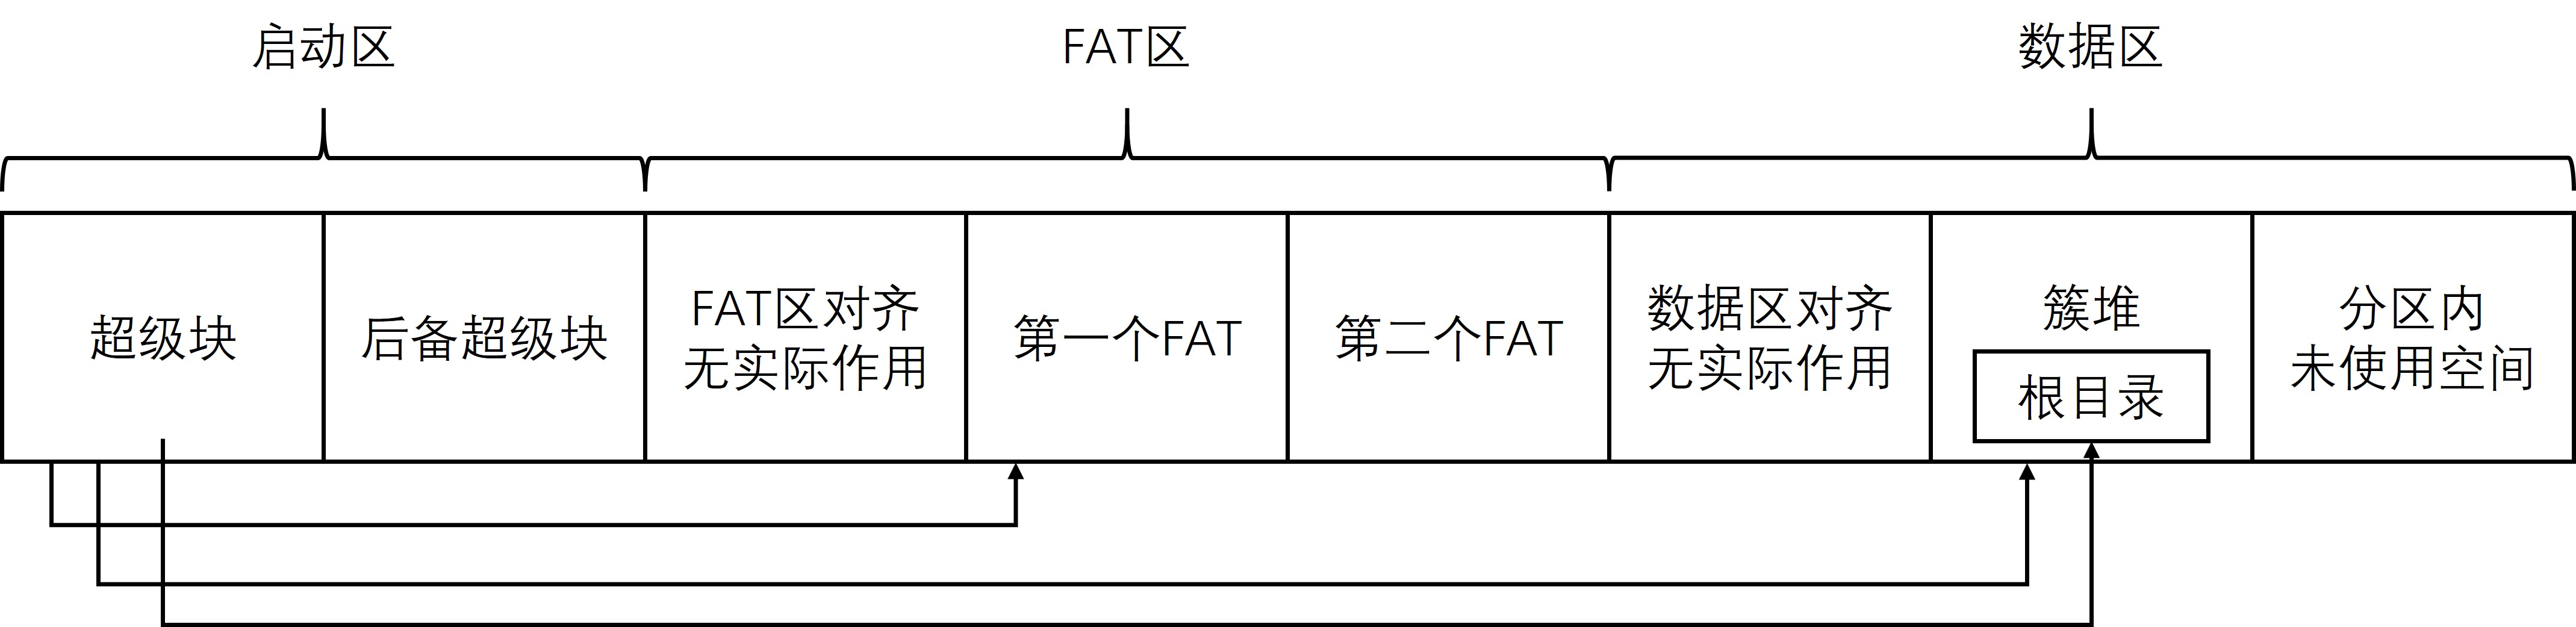
\includegraphics[width=\linewidth]{chap2_exfat_overview.pdf}
    \caption{exFAT 文件系统分区}
    \label{fig:exfat_overview}
\end{figure}

exFAT 文件系统在存储设备上的分区可以划分为三个主要部分:启动区、FAT 区和数据区,如图\ref{fig:exfat_overview}所示。
启动区包含超级块和后备超级块。
超级块(Superblock)中包含文件系统的基本信息,如扇区和簇的大小、FAT 区和数据区的位置、根目录所在簇等。
超级块一般位于存储设备上 exFAT 分区的起始位置,会在 exFAT 打开时被读取。
利用超级块中的信息,操作系统可以读取文件分配表并初始化根目录。
超级块对 exFAT 文件系统非常重要,因此还会安排一个后备超级块(Backup Superblock),以应对超级块损坏的情况。
如果超级块和后备超级块都损坏了,exFAT 文件系统将无法被挂载。

\subsection{FAT 表}\label{subsec:fat}
exFAT 将数据区里存储文件的部分(一般被称为簇堆,Cluster Heap)划分为一系列的簇(Cluster),
一个簇一般包含若干扇区。
扇区是存储设备的最小读写单元,而簇是文件分配的最小单元,即块设备上逻辑存储的基本单位。
作为 FAT 文件系统家族中的一员, exFAT 也使用文件分配表(FAT,File Allocation Table)\parencite{anderson2016fat}来组织文件。
文件分配表描述了簇和文件内容之间链接关系,位于启动区之后的 FAT 区,这个区域中可能存在一张或两张 FAT 表,
这个信息可以从启动区中的超级块得知。
若只存在一张 FAT 表,则这张表是主 FAT 表;若存在两张 FAT 表,两张表内容相同,第二张作为备份存在。

再说回到文件的组织,exFAT 文件系统中的一个文件可能由若干簇组成,这些簇组成了一个簇链。
exFAT 中允许的文件分配方式可能有两种,使用 FAT 进行分配和连续分配。
对于不使用 FAT 表的分配模式,即连续分配,文件会被组织成块设备上连续的簇,
这种情况下只需要获得文件的起始簇编号和文件的大小,即可得知文件内各个簇的编号。
而对于使用 FAT 的分配方式,文件分配表中维护了当前簇的下一个簇的编号。
这种 FAT 的组织结构类似链表,如果将一个文件中的一系列簇视作一个链表,
文件分配表中的条目相当于链表结构中的 Next 指针。
在读取某个文件时,通过查找文件分配表可以依次找到文件在磁盘上对应的各个簇的编号,从而访问文件的内容。
出于某些历史上的原因, exFAT 的簇编号从 2 开始,也就是说,假设数据区一共包括 $ N $ 个簇,第一个簇的编号是 2,
最后一个簇的编号是 $ N + 1 $。若从文件分配表中得到某个合法的簇编号 $ C $,该簇的物理编号是 $ C - 2 $。

\subsection{目录结构}\label{subsec:dentry}
数据区则是用于存储用户的文件和文件夹的区域,exFAT 文件系统内的所有文件和文件夹(包括根目录和系统文件)
的数据都存储在这个区域,并使用文件分配表来进行组织。
exFAT 使用目录树结构\parencite{al-turany2019understanding}来管理存于簇堆中的文件系统结构和文件。
在目录树中,父目录与子目录之间存在一对多的关系。
超级块中记录了文件系统的根目录所在簇,所有其他的目录都以单链方式从根目录派生。
每个目录由一系列目录项(Directory entry,在本文中简称为 Dentry)\parencite{wang2020research}组成,exFAT 中的单个目录项的大小固定为32字节。
事实上,exFAT 内的目录文件的文件内容就是一系列目录项。
一个或多个目录项可以组成一个目录项集(Directory entry set,在本文中简称为 Dentry set),
每个目录项集都描述了该目录下的一个子目录。

每一个有效的目录项可以按照属于主目录项或次目录项、属于关键目录项还是可选目录项分为四类。
每一个目录项集都是由一个主目录项和一系列次目录项组成,主目录项中会指明相关联的次目录项的个数。
关键主目录项包含一些对于 exFAT 文件系统的正确管理至关重要的信息,一个完整的实现应当支持所有这种类型的目录项。
可选主目录项的实现是可选的,这类目录项的作用是辅助管理文件系统,我们的实现中暂时并未支持这类目录项。
关键次目录项包含管理其所在目录项集的关键信息,虽然对任何关键次目录项的支持是可选的,但一个未识别的
关键目录项会使整个目录项集无法识别,我们的实现还是支持了 exFAT 标准中出现的所有关键次目录项。
可选次目录项的实现也是可选的,一个目录项集中出现的未识别的可选次目录项可以被忽略。
除此之外,exFAT 还定义了两种无效的目录项:未使用的目录项(Unused)和被删除的目录项(Deleted)。
表\ref{tab:dentry}中列出了我们的实现中主要的 Dentry 类型。
\begin{table}[h]
    \centering
    \begin{tabularx}{\textwidth}{|c|c|Y|}
    \hline
    Dentry类型 & 种类 & 描述 \\
    \hline
    Bitmap & 关键主目录项 & 与系统文件 Bitmap 关联的目录项,位于根目录中,没有次目录项,Bitmap用于跟踪磁盘上的空闲簇和已分配簇\\
    \hline
    Upcase Table & 关键主目录项 & 与系统文件大写转换表(Upcase Table)关联的目录项,位于根目录中,没有次目录项,大写转换表用于支持exFAT对大小写不敏感的特性\\
    \hline
    File & 关键主目录项 & 描述文件和目录的信息,合法的 File 目录项后会跟着一个 Stream 目录项和至少一个 Name 目录项\\
    \hline
    Stream & 关键次目录项 & 补充描述文件和目录的信息,紧跟 File 目录项出现\\
    \hline
    Name & 关键次目录项 & 记录相关文件和目录的名称,紧跟 Stream 目录项出现\\
    \hline
    Vendor Extension & 可选次目录项 & 文件供应商自定义目录项,只能出现在 Stream 和 Name 目录项之后\\
    \hline
    Vendor Allocation & 可选次目录项 & 文件供应商自定义目录项,只能出现在 Stream 和 Name 目录项之后\\
    \hline
    Unused & - & 未使用的目录项,只能出现在所在目录的末尾\\
    \hline
    Deleted & - & 被删除的目录项\\
    \hline
    \end{tabularx}
    \caption{Dentry 类型}
    \label{tab:dentry}
\end{table}



\section{页缓存及数据预取}
页缓存(Page Cache)\parencite{tanenbaum2014modern}\parencite{ostep}\parencite{bovet2005understanding}和
数据预取(Readahead)\parencite{readahead}\parencite{sequential_prefetching}是两种被广泛应用的技术,
用于解决磁盘驱动器的特性与应用程序访问模式之间的巨大差距,从而提高数据访问的效率。

首先,我们需要了解这种差距的来源。
磁盘驱动器在处理大规模顺序读写请求时表现优秀,但在定位数据(Seek)上效果不佳。
相对应的,应用程序却倾向于进行大量的小规模读写。\parencite{disk_performance}\parencite{disk_io_behavior}
这就产生了一个问题:如何解决磁盘驱动器的特性与应用程序访问模式之间的不匹配?

这时,页缓存和数据预取的作用就显现出来。
页缓存是一种加速数据访问的技术,它利用应用程序访问数据的局部性特点,
将常用的文件数据缓存至内存中,从而加快应用对文件数据的访问速度。

但如果仅使用页缓存来缓存应用访问过的数据,数据被首次访问时仍然需要从磁盘上读取,
不可避免的带来磁盘读写的延迟。
在某些特定场景下,数据只会被应用访问一次(如顺序遍历),此时页缓存将完全无法发挥其优势。
为了使得磁盘读写的延迟能够对应用程序最大程度上隐藏,人们又发明了数据预取技术。
数据预取是一种预测性的技术,它依据应用过去的访问模式来预测未来可能需要的数据,
并在数据被需要之前提前从磁盘上读取这些数据到页缓存中,尽可能以大块的方式进行。
当这些数据真正被访问时,由于它们已经在内存中可用,就能避免了磁盘访问的延迟。

通过结合使用页缓存和数据预取,对于有明显访问模式的应用(如顺序访问),我们可以显著提高应用程序的性能。
这两种技术共同解决了磁盘驱动器的特性与应用程序访问模式之间的不匹配问题,使数据访问更加高效。


% vim:ts=4:sw=4
